% !TEX root = mythesis.tex

%==============================================================================
\chapter{Detector exposure and Limits to the diffuse flux}
\label{sec:align}
%==============================================================================
 
The chapter aims to detail the procedure used to calculate the detector exposure or sensitivity to neutrinos for the DG$\mathrm{_{low}}$ region. The efficiencies calculated in the last chapter are used and the final expected neutrino rates are calculated. The first part of the chapter describes the exposure calculation along with the exposure contribution from different channels. Systematic uncertainties which can arise during the full analysis along with their contribution to the exposure are also discussed. 
The second part of the chapter details the results of the unblinding where no possible neutrino candidates were found for the angular range. Using this information an upper limit on the incoming flux of UHE $\nu$ is calculated. This limit is further compared to the one obtained by the previous analysis for the same time period but without the contribution of new triggers. The overall improvement forms a crucial result of this work. 


\section{Exposure Calculation}
\label{sec:det_exposure_calc}

One of the most accurate techniques used at Auger to calculate the exposure of the SD array to UHE$\nu$ is through extensive simulations of different detector configurations. In this method MC neutrino showers are thrown over varied detector configuration to calculate the effective or active area at each instant of time. Since the detector configuration of the SD array is constantly changing(\textit{faulty tanks, regular maintenance etc.}), sometimes on a daily basis, this technique requires a large amount of computational time and resources making it less desirable for use in this analysis. 

In this analysis, a different approach based on the 6T5 condition, which is required for each selected event in this analysis, is used for the exposure calculation. For this calculation, the 6T5 hexagon is taken to be the smallest possible detection unit for the $\nu$ event. The effective area i.e. the area seen by the incident cosmic neutrino for this detection unit at full efficiency is given by the Brillouin area~\cite{PierreAuger:2010zof}, $A_{6T5} = 1.95km^2$ as shown by the shaded area in fig~\ref{}. The aperture for this detector unit is dependent on the energy of the primary neutrino ,the slant depth in the atmosphere, X, neutrino flavor, type of the interaction, zenith angle, azimuth angel and the point of impact of the shower on the ground. The effective \textit{acceptance} of the detector unit can be written as follows:

\begin{equation}
  \label{eq:nu_accep}
  A_{hex}(E_{\nu}, X)  = \int^{\phi = 2\pi}_{\phi = 0} \,d\phi \int_{\theta_{min} = 58.5^{\circ}}^{\theta_{max}= 76.5^{\circ}}  \, A_{6T5} \cdot \varepsilon(E_{\nu}, X, \theta) \cdot sin\theta cos\theta \cdot d\theta    \mathrm{[cm^2 sr]}
\end{equation}

,where $\varepsilon(E_{\nu}, X, \theta)$ is the neutrino detection efficiency for each simulated energy, slant depth and zenith discussed in the last chapter. An example for a particular combination is given in fig.~\ref{}. Plots for efficiency for each combination can be found as part of the git code made available for this analysis. 

The next step involves integrating the \textit{acceptance} over the different simulated injected slant depths (as given in table~\ref{tab:Simulation_params}). This accounts for the \textit{effective mass} target for the neutrino identification over the 6T5 hexagon unit. It is calculated as follows. 

\begin{equation}
  \label{eq:nu_eff_mass}
  M_{hex}(E_{\nu}) = \int_X A_{hex}(E_{\nu}, X) \cdot dX
\end{equation}

Fig.~\ref{} shows the effective mass for both CC and NC interaction channels for a single 6T5 hexagon unit. Like the detection efficiency it increases with energy. 

Exposure calculation still needs to account for the detector configuration and its evolution over time. We reduced our array to units of 6T5 hexagons and a full SD array consisting of 1660 stations consists 1420 of these hexagons. Since the establishment of the Pierre Auger Observatory the active number of 6T5 hexagons are monitored every second. This forms a very good indicator for the time evolution of the SD array since any non-working station or large periods of instability are intrinsically recorded in the number of active 6T5 hexagons at that time. The instantaneous number of hexagons, $n_{hex}(t)$ thus can be used as an indicator of detector configurations over time. The $n_{hex}(t)$ were updated and calculated every minute and have an uncertainty of about 1.5\% as mentioned in~\cite{PierreAuger:2010zof}. To calculate the energy dependent exposure, the effective mass of one 6T5 hexagon is multiplied by the instantaneous number of hexagons and integrated in time. Further, the $\nu$ interaction probability for each flavour(i = $\nu_e, \nu_{\mu}, \nu_{\tau}$) and channel(c = CC, NC) is also folded in. The exposure is given as:

\begin{equation}
  \xi^{i,c}(E_{\nu}) = \frac{\sigma^{i,c}(E_{\nu})}{m_N} \int_{t} M_{hex}^{i,c}(E_{\nu}) \cdot n_{hex}(t) \cdot dt =  \frac{\sigma^{i,c}(E_{\nu})}{m_N} \cdot M_{hex}^{i,c}(E_{\nu}) \cdot N_{hex}
\end{equation}

,$\sigma^{i,c}(E_{\nu})$ is the neutrino nucleon cross-section~\cite{Cooper-Sarkar:2011jtt} and $N_{hex}$ is the total number of active 6T5 hexagons integrated in time over the search period. The value for $N_{hex}$ calculated for the period analysed is . The energy dependent exposure for different flavors and interaction channels is shown in fig~\ref{fig:Exp_flavors_comp}. It is necessary to point out again that the double bang showers which can be produced by $\nu_{tau}$ are not taken into account for this analysis which was also mentioned in sec.~\ref{sec:sim_DGL} 

\begin{figure}[t!]
  \centering
  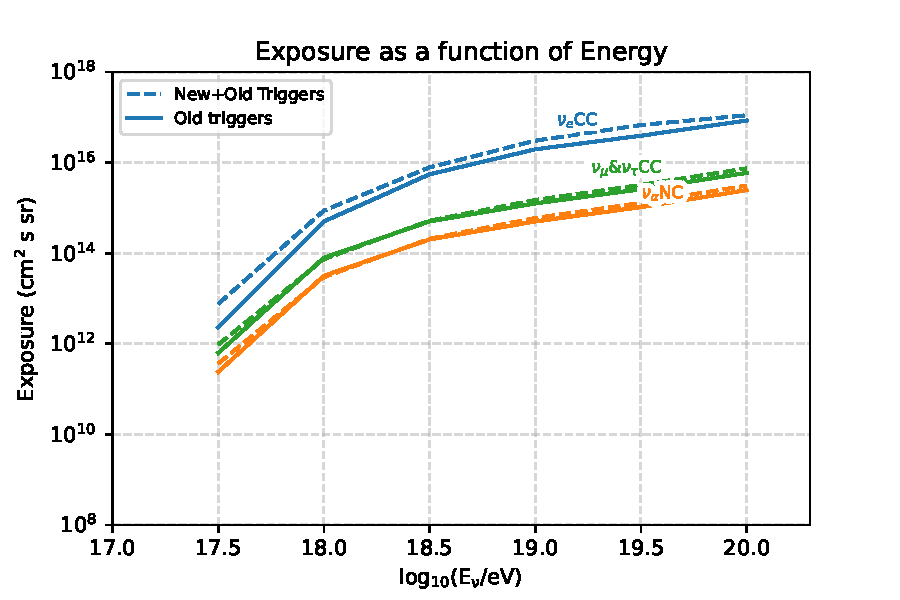
\includegraphics[width=14.5cm]{thesis_figures/ExpLimits/Exposure_comp_all_anotated_new_sim_optim.pdf}
  \caption{Exposure different channels}
  \label{fig:Exp_flavors_comp}
\end{figure}

An effective or total exposure, $\xi_{tot}(E_{\nu}) = \sum_{i}\sum_{c} \xi^{i,c}(E_{\nu})$ is calculated by summing all the interaction channels and assuming a 1:1:1 flavour ration at earth(large propagation distances combined with neutrino oscillations) as shown by the red line in fig~\ref{fig:Exp_total_comp}. 

\begin{figure}[t!]
  \centering
  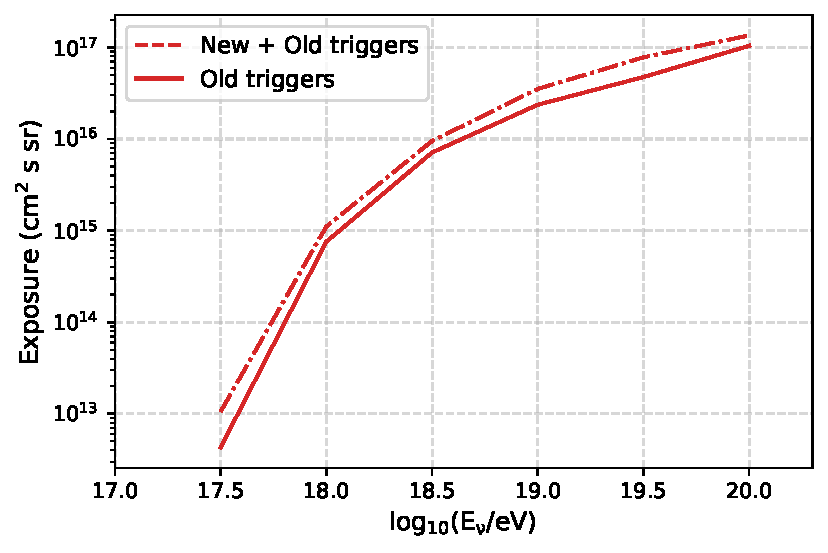
\includegraphics[width=14.5cm]{thesis_figures/ExpLimits/Exposure_comp_total_new_sim_optim.pdf}
  \caption{Total exposure}
  \label{fig:Exp_total_comp}
\end{figure}

As seen in the figure the $\nu_e$ CC channels contributes the most to the total neutrino exposure($\sim$85\%). The exposure rises rapidly at lower energies and then mostly flattens with just a slight increase which is due to the energy dependent neutrino cross-section. The shape is due to the neutrino detection efficiency which is small at lower energies as shown in fig~\ref{} in the last chapter. The next dominant channels are the $\nu_{\tau}$ and $\nu_{\mu}$ which have a similar detection efficiency as the NC channel but have a higher value of cross-section. The NC channel contribution is very small($\sim$5\%) due to the reasons discussed in section ~\ref{subsec:nu_sel_nudeteff}.  

The exposure calculated this analysis is compared to the one calculated using the previous analysis for the same time period in fig~\ref{fig:Exp_flavors_comp}. For the CC channel a 5x improvement is seen at lower energies and a 2x improvement at higher energies. For NC this improvement is not that significant. There is a 2x improvement at lower energies and a 1.5x improvement at higher energies. The improvement at lower energies is due to the inclusion of the new triggers MoPS and ToTd which enhance the detection efficiency at lower energies. The improvement at higher energies is mainly due to the improved Fisher analysis. The total exposure is also improved by a factor of ... 

\section{Systematic uncertainties}
\label{sec:det_uncert}
\todo{Determine what to write}
HERWIG PYTHIA difference take from old analysis.
PDF difference what is this ?
Hadronic interaction calculate yourself for 72 deg and $10^{19}$eV
https://scipost.org/SciPostPhysProc.13.028/pdf for CORSIKA vs others.
GAP2010-027 sytematic uncertainities neutrinos 
Also consider tau energy Loss maybe already mentioned in 2010 neutrino paper. 
Offline fluctuations and different reconstruction algorithms quote your own work.
can also quote An improved limit to the diffuse flux of ultra-high energy neutrinos
from the Pierre Auger Observatory(doi:10.1103/PhysRevD.91.092008) 
\section{Data unblinding}
\label{sec:data_unblinding}
As mentioned before in section~\ref{subsec:nu_sel_samp} the search data comprises of all events recorded at the Observatory between 2014-2021 which have a SD ID number non-divisible by 5 i.e. 80\% of all SD data recorded between 2014-2021. This search data sample was further split into a 20\% test sample similarly where SD ID numbers divisible by 4 were taken to be a part of the test sample while the rest became the part of the 60\% search sample. This split was done to perform the unblinding in two stages. The first where only the test sample in unblinded to detect any flaws with the analysis and if and when those flaws are fixed, the rest of the data is unblinded. This exercise turned out to be useful as a slight flaw was uncovered during the unblinding process of the 20\% test sample which was corrected. Said flaw which is described in more detail later required the whole reconstruction process along with the training of the Fisher polynomial to be performed again. This also led to the unblinded 20\% test sample to be blinded again since the reconstruction was altered. The splitting procedure was repeated and the total unblinding was performed again in parts. It is important to mention in all of unblinding procedure \textbf{0 neutrino events survive} the analysis selection.
This section is thus split into two subsections. The first describing the unblinding of the 20\% test sample along with the changes brought about by this unblinding. The second section details the full unblinding of the redone search samples (test + remaining) and discusses the interesting features of the unblinded search samples. 

\subsection{20\% test sample}
\label{subsec:unblind_20}

\todo{Test sample before the reco changes:}
% \begin{figure}[t!]
%   \centering
%   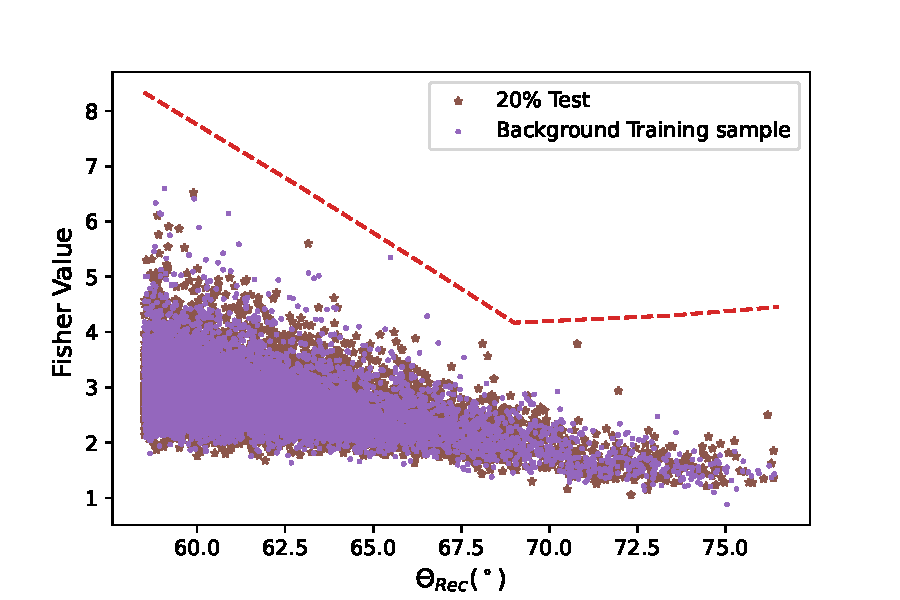
\includegraphics[width=14.5cm]{thesis_figures/Nu_analysis/Fisher_plots/Fisher_comp_bkg_test_wnt.pdf}
%   \caption{Test_reval vs background}
%   \label{fig:Fish_bkg_test}
% \end{figure}

The Fisher value distribution for the test sample is shown in fig~\ref{}. As it is shown no event passes the Fisher cut in any angular region. However, there are a few events which come very close to the cut line. Five events marked with a red circle were analysed in more detail. Each of them has its own unique reason with only the one with zenith~ being the most interesting. This event has the ID of 66106356. After looking at detailed information about the event it was found out that the accidental station cut used is insufficient. Previously, the  accidental cut (rejection of stations with Totalsignal < 3 VEM) is only applied to the event if there are more than 5 stations in the event. Since for this analysis due to the inclusion of MoPS and ToTd an overall increase in events is expected which also increases the overall number of stations with accidental stations this cut needs to be reduced a bit to take this overall increase into account. Thus, this cut was reduced to apply for events with more than 4 stations. This reduction of the cut decreases the total events passing the analysis cut by $\sim$5\% for the background training sample and $1-2$\% for the signal training sample. The Fisher coefficients and cut changes slightly. After this change in the reconstruction the test sample was obtained again and compared to the background dample as shown in fig~\ref{fig:Fish_bkg_test}. The other interesting events which have $\mathcal{F}$ values close to the $\mathcal{F_{cut}}$ with their respective ids are tabulated in table~\ref{}. These events were individually evaluated. Some of these () were found to have a bad time residual fit primarily because of multiple peaks observed in stations triggered by the new triggers. Since, no segmentation algorithm was used for stations with MoPS and ToTd triggers sometimes a wrong peak was selected which affected the reconstruction for these events. A future analysis with a corrected segmentation algorithm which is functional for the new triggers MoPS and ToTd is envisaged in the future analysis upgrades. Such events are expected to be limited to less than $\sim$1\% of total events but still require a careful look for future analysis upgrades. A further detailed analysis was also performed for these events where the primary mass composition was extracted via the muon production distributions as mentioned in~\cite{PierreAuger:2014zay}. Even with large uncertainties these events are most likely due to a light deep primary. For the other three events no particular feature worth mentioning was observed. 

\begin{figure}[t!]
  \centering
  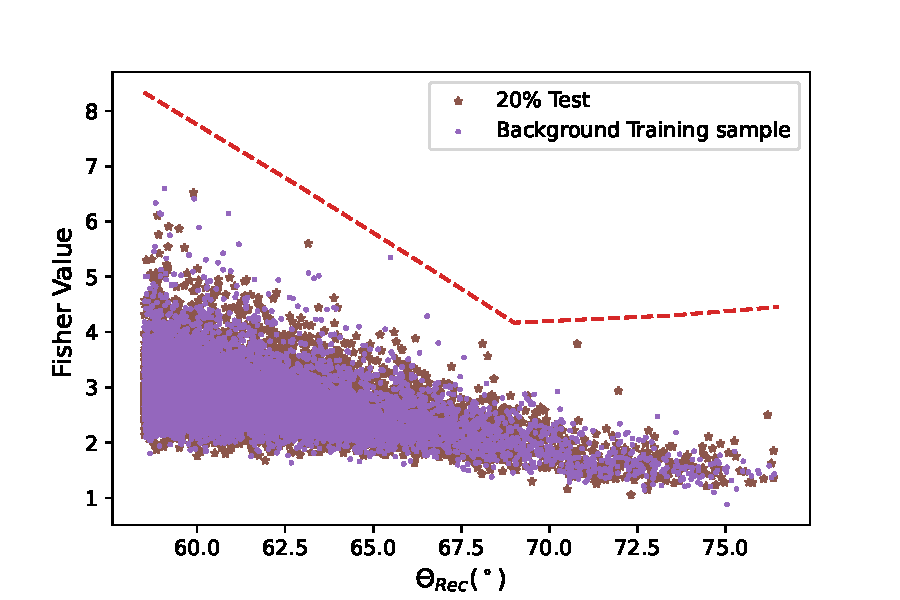
\includegraphics[width=14.5cm]{thesis_figures/Nu_analysis/Fisher_plots/Fisher_comp_bkg_test_wnt.pdf}
  \caption{Test_reval vs background}
  \label{fig:Fish_bkg_test}
\end{figure}

\begin{figure}[t!]
  \centering
  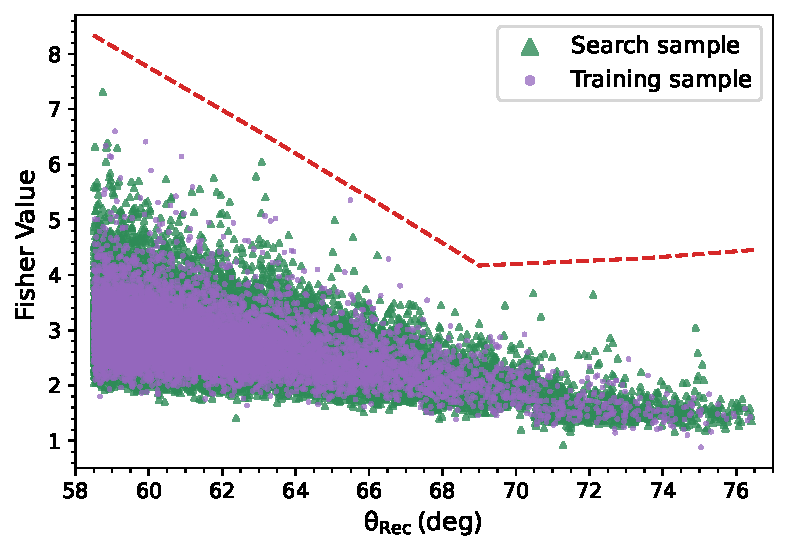
\includegraphics[width=14.5cm]{thesis_figures/Nu_analysis/Fisher_plots/Fisher_comp_bkg_search_wnt.pdf}
  \caption{Search vs background}
  \label{fig:Fish_bkg_test}
\end{figure}

\subsection{Reevaluated 20\% test search sample and 60\% search sample}
\label{subsec:unblind_60}
After the unblinding of the test sample and changing the cut mentioned in the section above, the unblinding was again performed in two stages. Initially a 20\% part was unblinded and then the remaining 60\% blinded sample was analysed. Again \textbf{0 neutrino candidates} were found after candidate selection. The results of the unblinding for each sub-angular bin is presented in fig~\ref{fig:Fisher_cut_2} along with the Fisher value as a function of zenith angle presented in fig~\ref{}. The results (red) are overlaid over the training(orange) and test (blue) samples with the dashed lines indicating the value of the $\mathcal{F_{cut}}$ obtained according to eq.~\ref{eq:fisher_poly_cut}. As it can be seen the distributions are compatible to each other within statistical fluctuations. The overlay also confirms that the exponential tail assumption is a reasonable enough to determine the $mathcal{F_{cut}}$. The goodness of the fit is once against presented in tab.~\ref{tab:Cut_eval_unblind} in the form similar to table~\ref{tab:Cut_eval}. This time for the observed values the numbers are calculated from the much larger search sample. It is found that the tails of the distributions which typically seemed to have fit badly also fit reasonably well. The events in the search sample that have $\mathcal{F}$ values close to the $\mathcal{F_{cut}}$ were again carefully checked and were found to be either due to the issues with the segmentation algorithm or known issues such as partial shower containment or large number of non-working PMTs both issues have also been seen in previous analysis. 

\begin{figure}[h!]
  \centering
   \begin{subfigure}[l]{.48\textwidth}
     \centering
     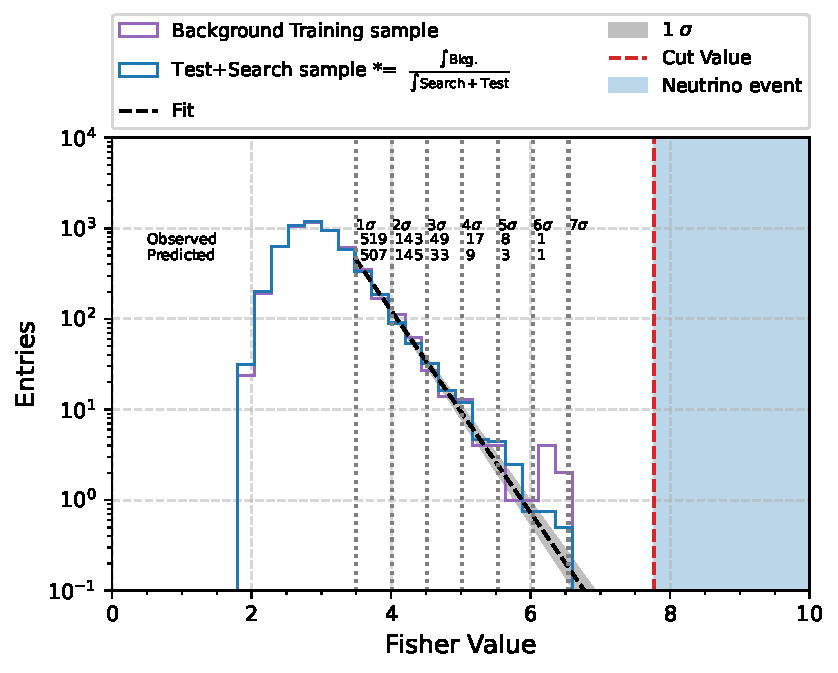
\includegraphics[width=\linewidth]{thesis_figures/Nu_analysis/Fisher_plots/Fisher_fit_search+test_bkg_region_58.5_61.5.pdf}
     \caption{58.5 61.5}
     \label{fig:58.5-61.5}
   \end{subfigure}
   %\hfill
   \begin{subfigure}[r]{.48\textwidth}
     \centering
     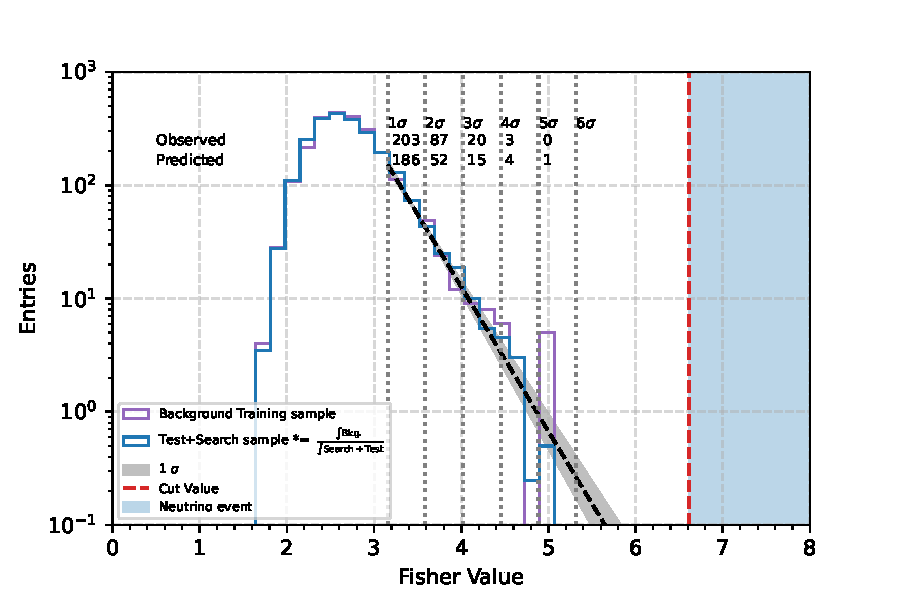
\includegraphics[width=\linewidth]{thesis_figures/Nu_analysis/Fisher_plots/Fisher_fit_search+test_bkg_region_61.5_64.5.pdf}
     \caption{61.5 64.5}
    \end{subfigure}
    \hfill
    \begin{subfigure}[l]{.48\textwidth}
      \centering
      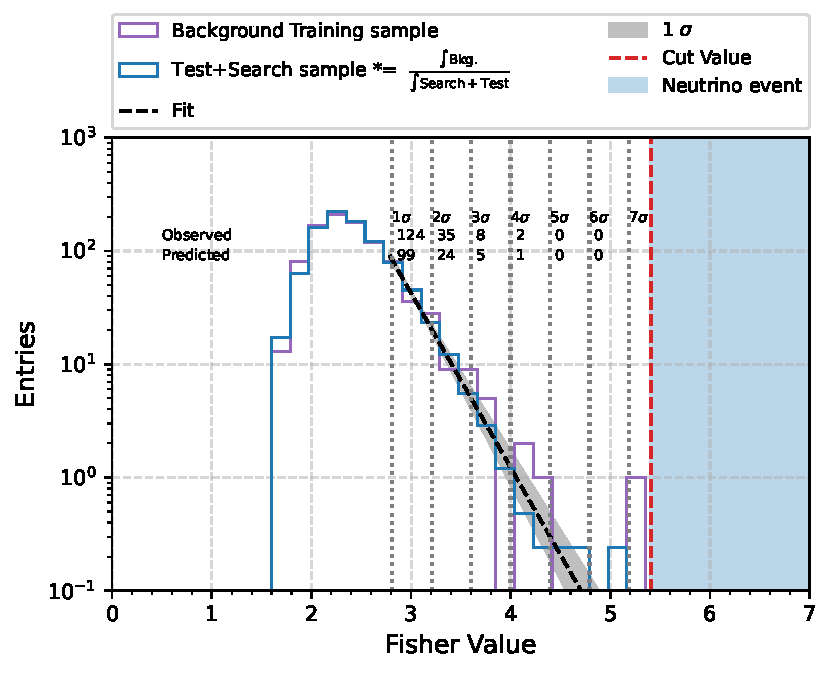
\includegraphics[width=\linewidth]{thesis_figures/Nu_analysis/Fisher_plots/Fisher_fit_search+test_bkg_region_64.5_67.5.pdf}
      \caption{64.5 67.5}
    \end{subfigure}

    \begin{subfigure}[r]{.48\textwidth}
      \centering
      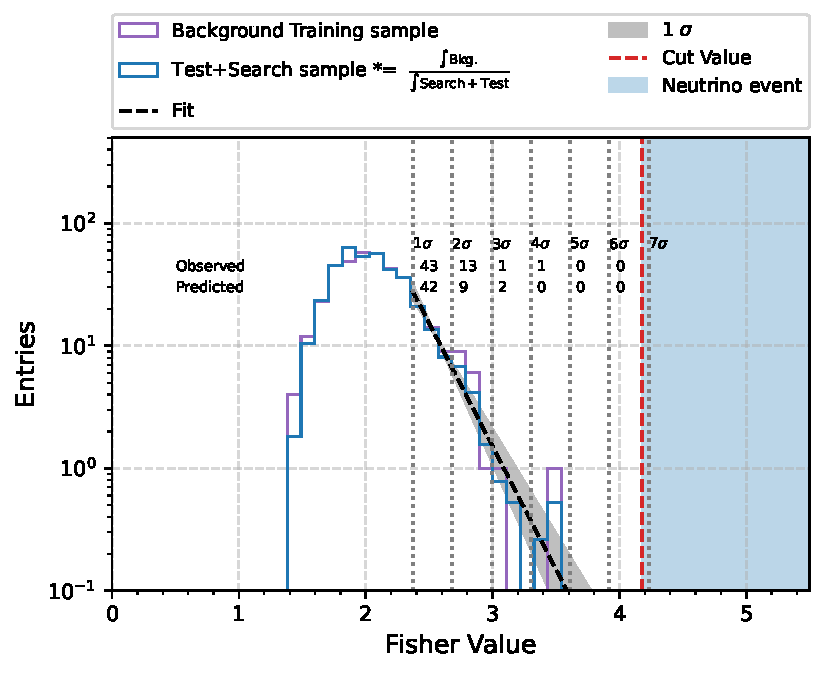
\includegraphics[width=\linewidth]{thesis_figures/Nu_analysis/Fisher_plots/Fisher_fit_search+test_bkg_region_67.5_70.5.pdf}
      \caption{67.5 70.5}
    \end{subfigure}
    \hfill    
    \begin{subfigure}[r]{.48\textwidth}
      \centering
      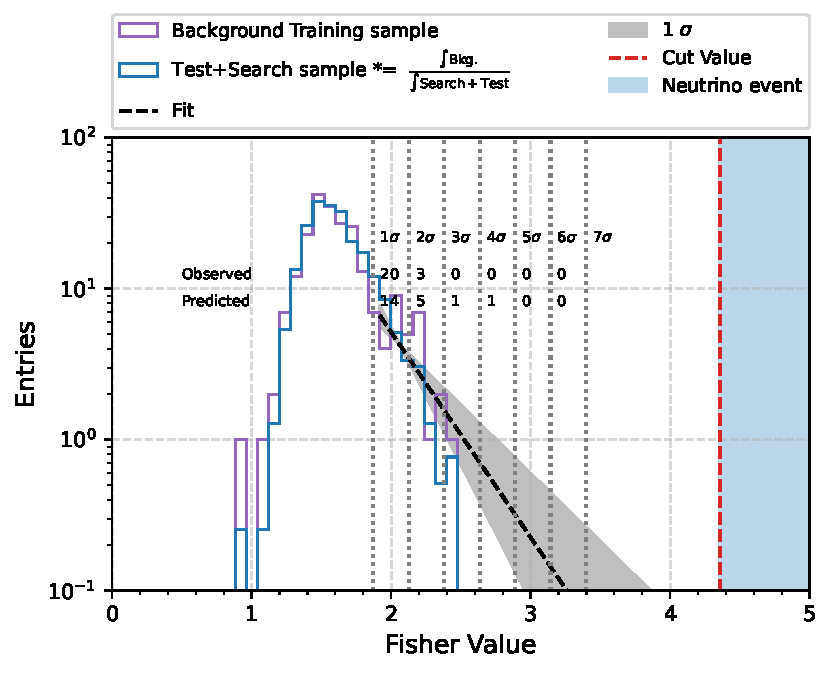
\includegraphics[width=\linewidth]{thesis_figures/Nu_analysis/Fisher_plots/Fisher_fit_search+test_bkg_region_70.5_73.5.pdf}
      \caption{70.5 76.5}
   \end{subfigure}
   \caption{Evaluating the goodness of fit of the Fisher cut for the search sample. The observed values are compared to the predicted values.}
    \label{fig:Fisher_cut_2}

\end{figure}

\begin{table}[h!]
  \centering
  \begin{tabular}{ |P{1.25cm}||P{2.4cm}|P{2.4cm}|P{2.4cm}|P{2.4cm}|P{2.4cm}| }
    \hline
      Fit & \multicolumn{5}{c|}{Number of events in $\mathcal{F}$ tails} \\
      Range & \multicolumn{5}{c|}{Observed - Predicted} \\
    \cline{2-6}
      & Region 1 & Region 2& Region 3& Region 4 & Region 5 \\
      &(58.5$^\circ$-61.5$^\circ$]&(61.5$^\circ$-64.5$^\circ$]&(64.5$^\circ$-67.5$^\circ$]& (67.5$^\circ$-70.5$^\circ$] & (70.5$^\circ$- 76.5$^\circ$] \\
    \hline 
    $\mu$ + 1$\sigma$ & 13 & 14 & 17 & 19 & 23 \\
    $\mu$ + 2$\sigma$ & 1640 & 1820 & 2040 & 2330 & 2720 \\
    $\mu$ + 3$\sigma$ & 140 & 220 & 140 & 230 & 120 \\
    $\mu$ + 4$\sigma$ & 140 & 220 & 140 & 230 & 120 \\
    $\mu$ + 5$\sigma$ & 140 & 220 & 140 & 230 & 120 \\
    $\mu$ + 6$\sigma$ & 140 & 220 & 140 & 230 & 120 \\
    \hline
  \end{tabular}
  \caption{Table to test captions and labels.}
  \label{tab:Cut_eval_unblind}
\end{table}
\section{Diffuse limit for the UHE neutrino flux}
\label{sec:diff_limit}
Since no neutrino candidate was found in this analysis, an upper limit to the flux of the incoming UHE$\nu_s$ can be evaluated. Let flux per unit area, \textit{A}, energy, solid angle $\omega$ and time be denoted by $\mathrm{\phi(E_{\nu}) = \frac{d^6 N_{\nu}}{dE_{\nu}d\omega dA dt}}$. The expected number of detected neutrinos can be calculated by folding in the total exposure $\xi_{tot}(E_{\nu})$ with flux as follows,

\begin{equation}
  \mathrm{N_{expected} = \int_{E_{\nu min}}^{E_{\nu max}} \phi(E_{\nu}) \cdot \xi_{tot}(E_{\nu}) \cdot dE_{\nu}}
\end{equation}

Assuming a differential UHE$\nu$ flux $\phi = k \cdot E_{\nu}^{-2}$, the integrated upper limit on the value of k is given by:

\begin{equation}
  \label{eq:integ_lim}
  \mathrm{k_{up} = \frac{N_{up}}{\int_{E_{\nu min}}^{E_{\nu max}} E_{\nu}^{-2} \cdot \xi_{tot}(E_{\nu}) \cdot dE_{\nu}}}
\end{equation}

, the value of $\mathrm{N_{up}}$ for a given confidence level can be determined based on the number of observed events and the number of expected background events. Different statistical methods can be used to obtain the value for $N_{up}$ based on the confidence interval. In the next sections some of these different statistical approaches are discussed in more detail. The Feldman and Cousins limit with an extension that incorporates the systematic uncertainties discussed above is chosen as a final estimate for $\mathrm{N_{up}}$.

\subsection{Feldman and Cousins limit}
\label{subsec:FandC}
Feldman-Cousins method~\cite{Feldman:1997qc} is a statistical technique used to construct confidence intervals, particularly for Poisson distributed data. This approach addressed the key shortcomings of traditional methods used to construct confidence intervals especially for cases where the number of observed events are low or zero. Traditional methods such as Gaussian approximation, which assumes that data follows a normal distribution which are used to calculate confidence intervals can often lead to incorrect interval particularly in rare event searches where the data is better described by a Poisson distribution. This can also lead to unphysical values e.g. negative value for rate of expected events. The Feldman-Cousins approach solves these problems by giving a unified method for constructing confidence intervals. The method ensures that the intervals are unbiased and do not favour one outcome over the other. It also ensures natural transition from two-sided intervals(where there is significant data) to one-sided upper limits(when there is little to no data). The method also respects physical constraints, such as non-negative value for expected event rates. It also provides intervals with more accurate coverage probabilities, reducing over-coverage issues common in other methods. 

The Feldman \& Cousins approach is implemented as a part of \textit{gammapy} in python~\cite{Gammapy:2023gvb} which was used  to get the interval for this analysis. The information was also verified with look-up tables in~\cite{Feldman:1997qc}. For a 90\% confidence interval, in case of zero signal and background events, the upper and lower limits are given as $N^{90\%}_{up} = 2.44$ and $N^{90\%}_{low} = 0$ respectively. If one signal event is seen with zero background then this interval shifts to [4.36,0.11]. It is important to note that both statistical and systematic uncertainties are not included for the intervals calculated in the Feldman \& Cousins method. 

\subsection{Rolke approach}
\label{subsec:Rolke}
The Feldman \& Cousins treatment is a frequentist method which requires the background source to be known precisely. Such a method can fail if the uncertainties are too high~\cite{Rolke:2000ij}. To solve this problem one can also use the Rolke method~\cite{Rolke:2004mj} which incorporates prior information in this case signal with a Poisson distribution and background with either a Poisson or Gaussian distribution. The method is implemented as a ROOT class under TRolke~\cite{TRolke_ROOT}. For a 90\% confidence interval in the case of zero signal and background events the interval is given as [2.21,0] assuming a Poisson distribution for both signal and background. As it is seen the interval is smaller in comparison to the Feldman \& Cousins approach. This can be explained much more clearly for the case where there is one signal event and no background where the Rolke interval is [3.65,0]. In this case according to the Feldman \& Cousins approach the event has to be a signal since the lower limit is > 0 but in the Rolke approach it is still possible that such an event in the signal region could be a background event i.e. in the Rolke approach the absence of background does not imply zero background, but it only means that the background is not too large. This is because background is treated as a Poisson number. Thus, the overall upper and lower limits in the Rolke approach are always smaller in comparison to the Feldman \& Cousins  method. 

\subsection{Conrad approach}
\label{subsec:Conrad}
The Conrad method for calculating confidence intervals allows the inclusion of systematic uncertainties in the evaluation. Using this approach the uncertainties in the background prediction, background detection and the signal detection efficiencies can be incorporated in the confidence interval calculation by integrating over the PDFs of these parameters~\cite{Conrad:2002kn}. The method computes the upper limit based on a likelihood ratio between the observed data and the null hypothesis(no signal). For this work the interval was calculated using POLE++~\cite{Conrad:2005zm} which is a C++ program that implements the Conrad method. The systematic uncertainty on exposure was estimated to be as [] as mentioned in section~\ref{sec:det_uncert}. Using a uniform PDF to characterise the exposure and a Gaussian assumption for background, for a 90\% confidence interval in the case of zero signal and background events the upper and lower limits are given as: 

\begin{equation}
  \label{eq:Conrad_lim}
  N^{90\%}_{up} = 2.39\\
  \, N^{90\%}_{low} = 0
\end{equation}

The interval is smaller in comparison to the Feldman \& Cousins method due to the uneven interval for the systematic uncertainty. For one signal event and zero background the interval changes to []. 

\subsection{Final calculation}
\label{subsec:final_lim}
After the determination of $N_{up}$ using the Conrad approach the equation~\ref{eq:integ_lim} can be solved to determine the upper limit to the diffused flux of UHE$\nu_s$. The integral goes from $E_min = 10^{17.5} $eV till $E_max = 10^{20.5} $eV which is the total energy range explored in the simulations. It is also important to note that the limit is only valid for a smaller energy window. The single flavour 90\% C.L. integrated limit is given by 
\begin{equation}
  \label{eq:final_lim}
  \mathrm{k_{90} < 6.3 x 10^{-17} GeV cm^{-2} s^{-1} sr^{-1}},
\end{equation}
It applies to an energy range of $E_{\nu} \epsilon [1.9 \times 10^{18} - 2.0 \times 10^{20}]$ which is the energy range for which $\sim$90\% total event rate is expected in the case of $E^{-2}_{nu}$ flux. The value along with the 90\% energy range is plotted as a solid line in fig~\ref{}.

\begin{figure}[t!]
  \centering
  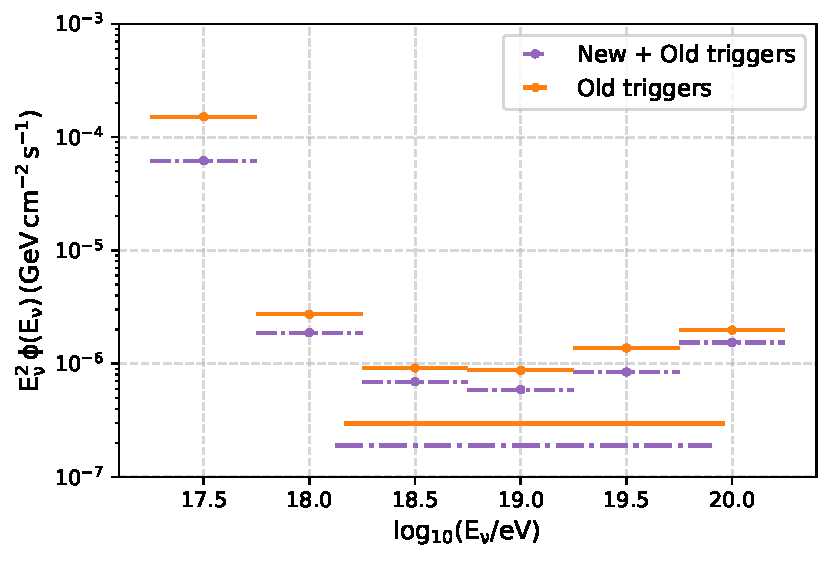
\includegraphics[width=14.5cm]{thesis_figures/ExpLimits/Integ_DiffLimit_comp_new_sim_optim.pdf}
  \caption{Diff limit new old comparison}
  \label{fig:Limit_comp_1}
\end{figure}

The other lines in green are the \textit{differential limits}. These are calculated by integrating the denominator of eq.~\ref{eq:integ_lim} in bins of width $\Delta = 0.5eV$ in $log_{10}(E_{\nu})$. Mathematically for the $i^{th}$ bin this can be represented as follows:

\begin{equation}
  \label{eq:diff_lim}
  \mathrm{Differential \,limit \, (i^{th} \, E_{\nu} \, bin)  = \frac{N_{Up}}{\int_{log_10(E^i - (\Delta log_{10}E)/2)}^{log_10(E^i + (\Delta log_{10}E)/2)} E^{-1}_{\nu} \cdot \xi(E_{\nu}) \cdot ln(10) \cdot d(log_{10}(E_{\nu}))}}
\end{equation}

Assuming constant exposure and flux in each energy bin the differential limit can be estimated as:

\begin{equation}
  \label{eq:diff_lim_approx}
  \mathrm{Approx. \, Differential \,limit \, (i^{th} \, E_{\nu} \, bin)  = \frac{N_{Up}}{E^{-1}_{\nu} \cdot \xi(E_{\nu}) \cdot ln(10) \cdot \Delta (log_{10}(E_{\nu}))}}
\end{equation}

These limits provide a way to denote the sensitivity of the detector for different energies. As it can be seen from the fig.~\ref{fig:Limit_comp_1} for the Down-going Low analysis the Pierre Auger Observatory is the most sensitive for energies $\sim$1 EeV. 

Both limits are also compared to the results from the previous analysis in fig~\ref{fig:Limit_comp_1}. As it was seen in the exposure comparison it is clear that the new triggers help improve the sensitivity at lower energies. For higher energies the improvements to the upper-limit for the diffuse flux of $UHE_{\nu_s}$ though not as signifivcant is still substantial. This improvement can be attributed to the changes in the Fisher analysis The integral flux limit sees an improvement $\sim$.. order of magnitude. The aim of this study was to evaluate the improvement, but it was always know that for this angular range significant improvements to the diffuse flux improvements were not expected. The diffuse flux limit and sensitivity for Auger is dominated by the Earth-skimming channel as shown in ~\cite{Aab_2019_diffuse}. This limit is significantly lower than the DG$\mathrm{_{low}}$ channel and is the main driver to constrain astrophysical and cosmogenic models. However, the improvements shown in this analysis are more important in the context of point source searches. This is discussed more in the next chapter. 

\begin{figure}[t!]
  \centering
  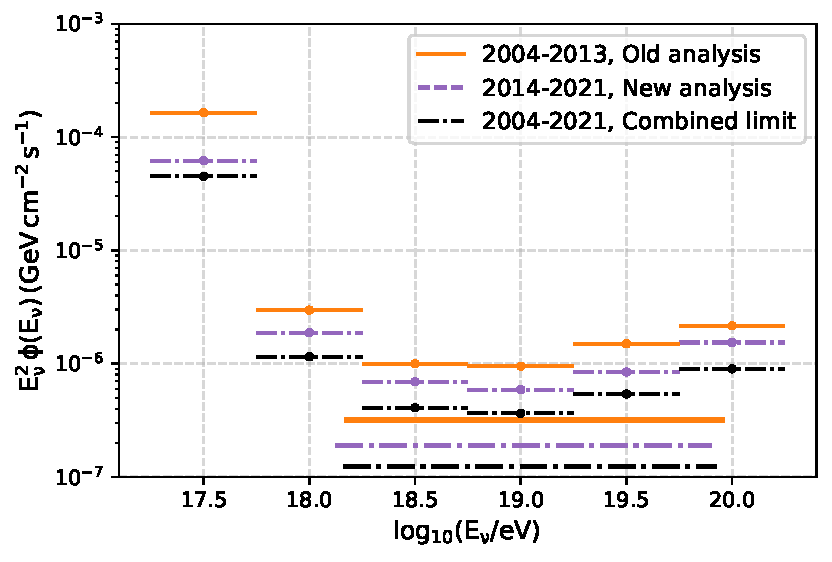
\includegraphics[width=14.5cm]{thesis_figures/ExpLimits/Integ_DiffLimit_comp_combined_new_sim_optim.pdf}
  \caption{Diff limit combination}
  \label{fig:Limit_comp_2}
\end{figure}

\begin{figure}[t!]
  \centering
  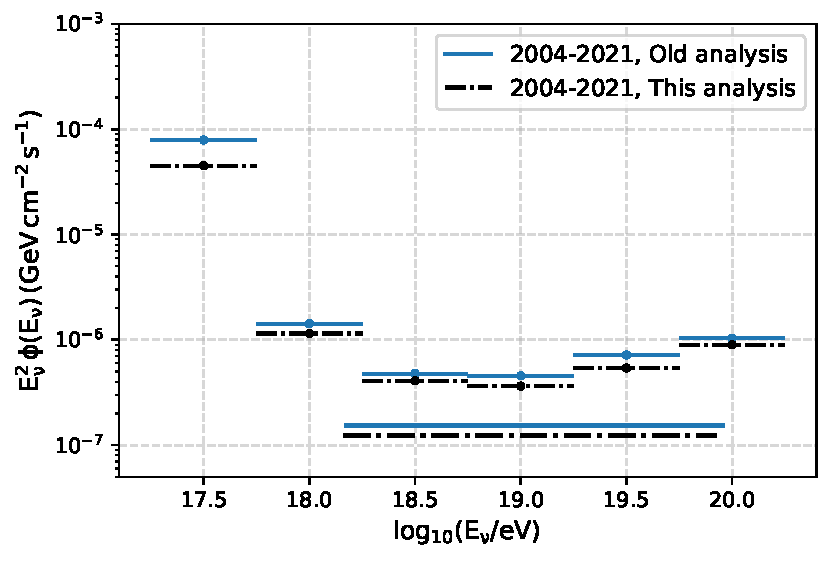
\includegraphics[width=14.5cm]{thesis_figures/ExpLimits/Integ_DiffLimit_comp_combined_new_sim_optim_3.pdf}
  \caption{Diff limit combination}
  \label{fig:Limit_comp_3}
\end{figure}


%%% Local Variables:
%%% mode: latex
%%% TeX-master: "mythesis"
%%% End:
